\newpage
\section{Text-to-Tree transformation}
\genHeader

As we shall see in a moment, libraries and shelves correspond to a folder structure while the contents for a single dictionary are specified in a file.
Figure \ref{fig:moca-4-Tokens} depicts a small sample of the textual syntax used to specify a dictionary. 

\begin{figure}[!htbp]
\begin{center}
 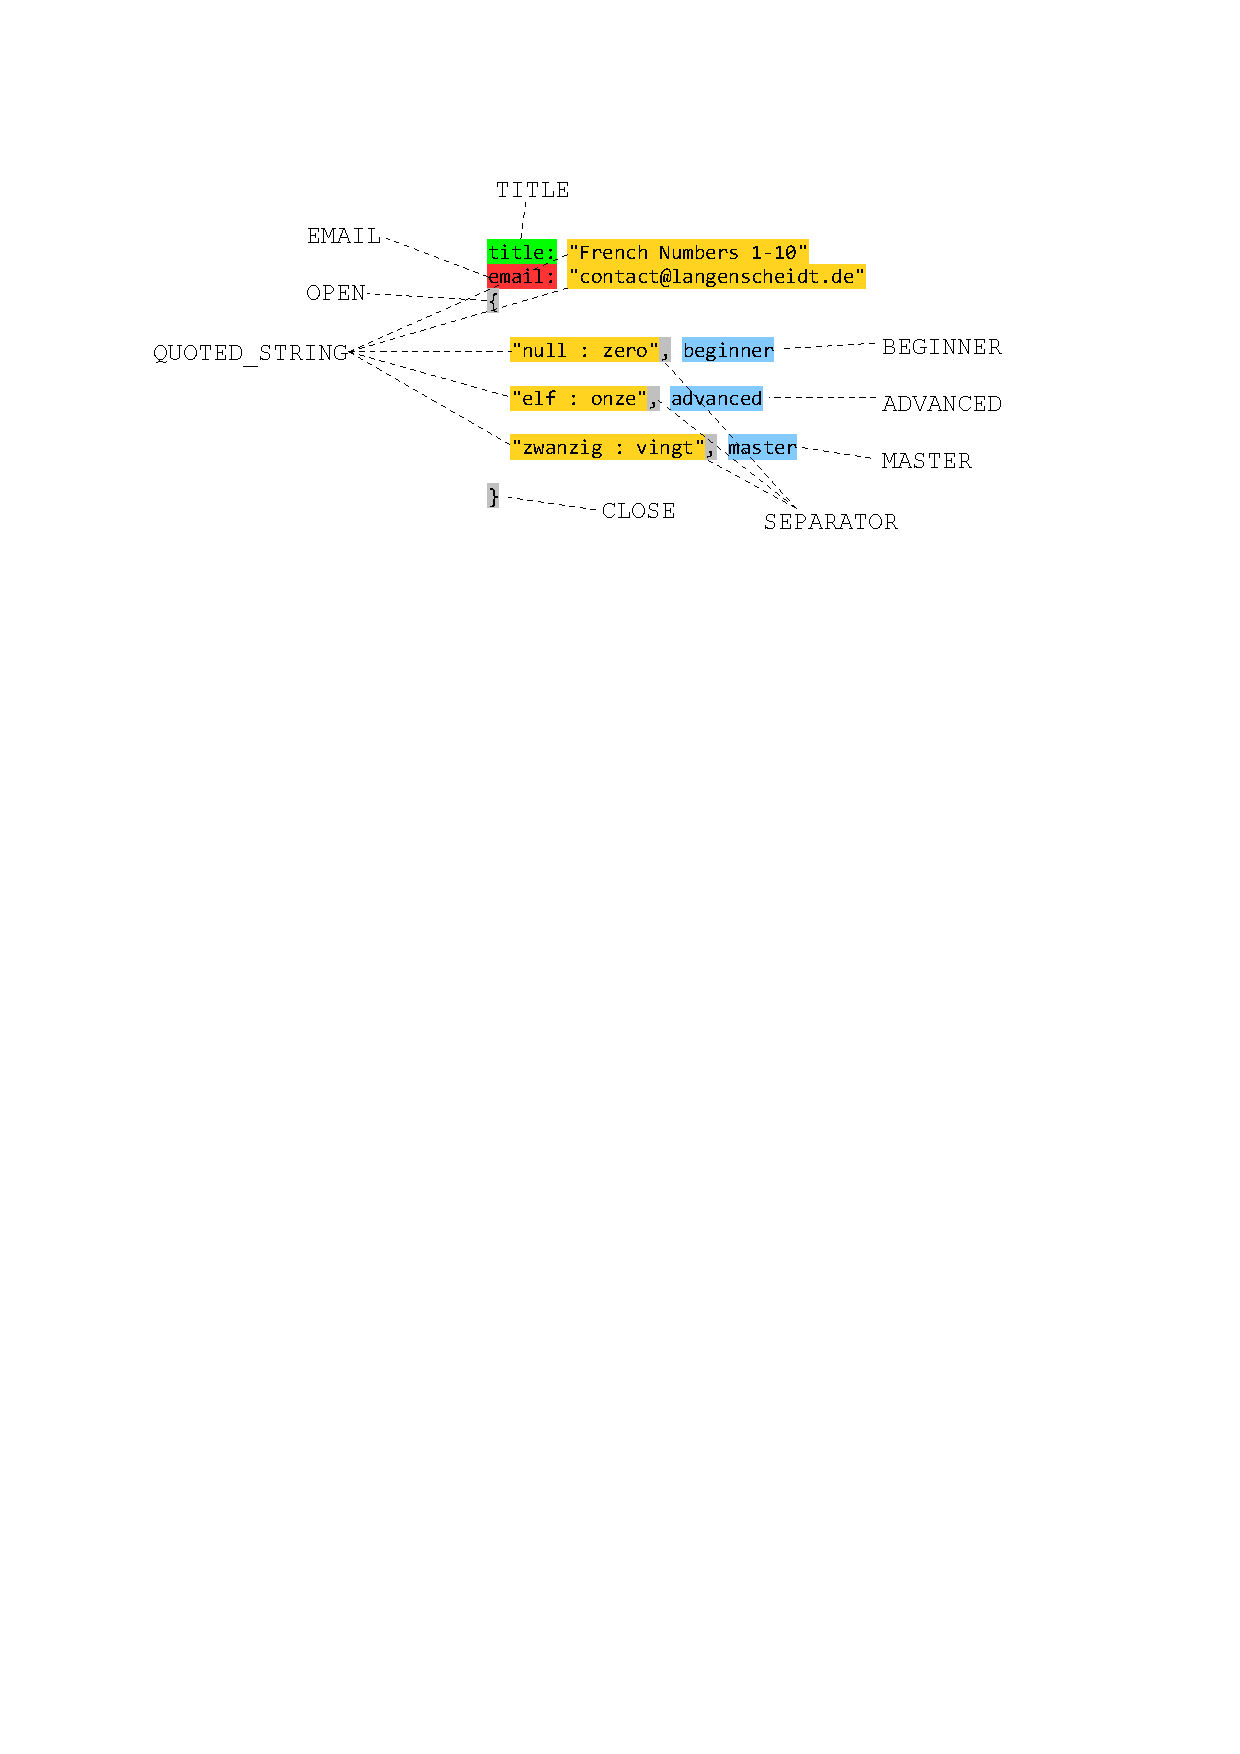
\includegraphics[width=0.7\textwidth]{4-tokens}
  \caption{Identified tokens in a dictionary file.}
  \label{fig:moca-4-Tokens}
\end{center}
\end{figure}

On the way to an instance model of our dictionary metamodel, the very first step is to create nice \emph{chunks} of characters. This step is called
\emph{lexing} and it simplifies the actual comprehension of the complete text. Interestingly human beings actually comprehend text in a similar manner, one
recognizes whole words without ``seeing'' every individual character. This is the reason why you can siltl raed tihs sneentce alsomt eforftlsesly. A lexer
recognizes these chunks or \emph{tokens} and passes them on as a token stream to the \emph{parser} that does the actual work of recognizing complex
hierarchical and recursive structures.
   
To recognize the tokens as indicated in Fig.~\ref{fig:moca-4-Tokens}, \texttt{ANTLR} can automatically generate a lexer in Java from a compact specification as
depicted in Fig.~\ref{fig:moca-6-lexer}. This is actually a DSL for lexing and is explained in detail in \cite{ANTLR}. If you do not know what EBNF is and have
problems understanding the lexer grammar then make sure you at least go through the documentation on \url{www.antlr.org} or read relevant chapters in
\cite{ANTLR}.

\begin{itemize}
  
\item[$\blacktriangleright$] When you first open \texttt{DictionaryLexer.g} it will have some comments that may help you but that you are free to delete if you
wish. In any case, Edit \texttt{DictionaryLexer.g} so it closely resembles Fig.~\ref{fig:moca-6-lexer}. You'll need to add the \texttt{import
org.moflon.moca.MocaUtil} statment to the header. For the rest of the file, be careful to avoid any typos and mistakes! Save the file to compile it, and ensure
no errors persist.

\end{itemize}
\newpage

\begin{figure}[!htbp]
\begin{center}
  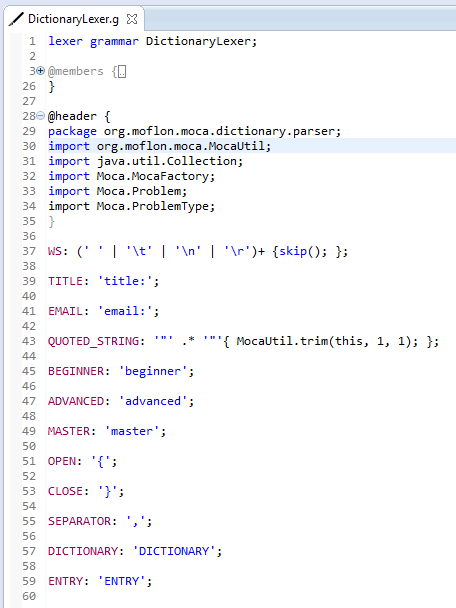
\includegraphics[width=0.8\textwidth]{eclipse_dictionaryLexer}
  \caption{Lexer grammar}
  \label{eclipse:dictionaryLexer}
\end{center}
\end{figure}

Now that we have our lexer built, the next step is to form the stream of tokens from the lexer into a \emph{tree}. In this context, a \emph{tree} is an acyclic,
hierarchical, recursive structure as depicted in Fig.~\ref{eclipse:dictLexer}. Depending on what the tree is to be used for, it can be organized much differently
with extra \emph{structural} nodes such as \texttt{DICTIONARY} or \texttt{ENTRY} that were not present in the textual syntax and are used to give additional
meaning to the tree.

\begin{figure}[htp]
\begin{center}
 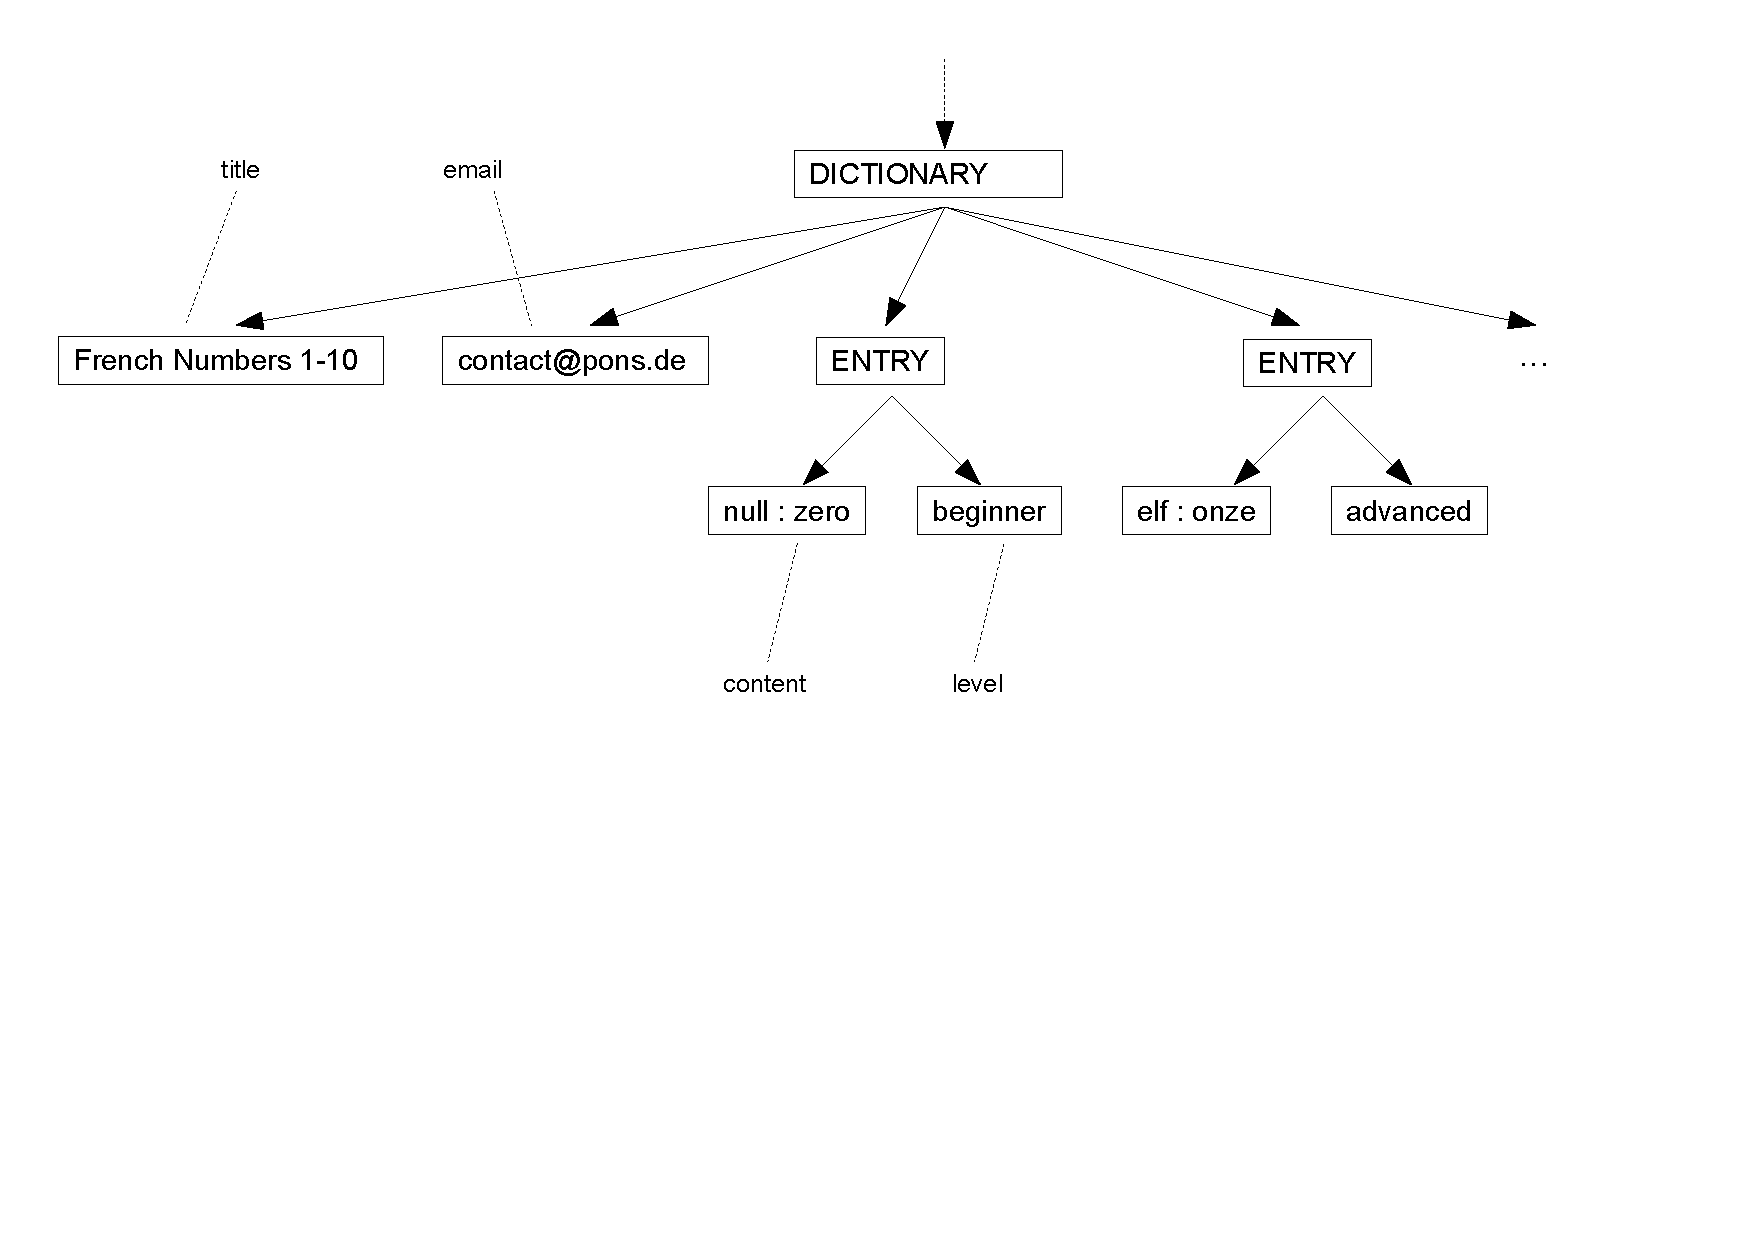
\includegraphics[width=\textwidth]{5-tree}
  \caption{MocaTree structure}
  \label{eclipse:dictLexer}
\end{center}
\end{figure}

\begin{itemize}

\item[$\blacktriangleright$] Open and edit \texttt{DictionaryParser.g} so it closely resembles Fig.~\ref{eclipse:dictParser}. It too has some comments that you
may remove, but you won't need to make any changes this time to \texttt{@header}. As with the lexer, avoid typos and mistakes and ensure it compiles before
proceeding.

\end{itemize}

\begin{figure}[!htbp]
\begin{center}
 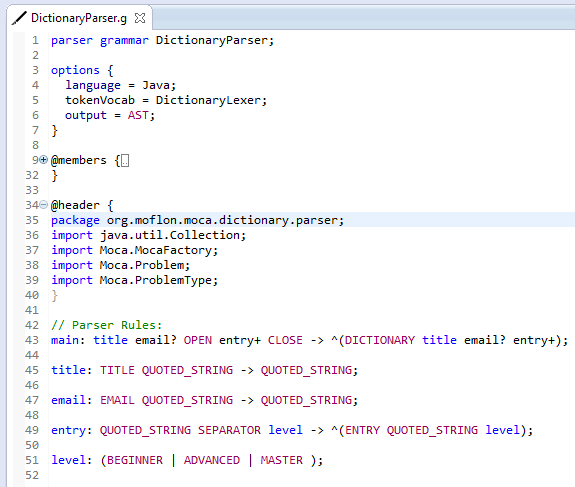
\includegraphics[width=0.9\textwidth]{eclipse_dictionaryParser}
  \caption{Parser grammar}
  \label{eclipse:dictParser}
\end{center}
\end{figure}

As you can see, the parser grammar is quite similar to the lexer grammar, but there are \emph{parser actions} after the \texttt{->} symbol, which build up the
tree. Using this simple tree language, one can (1) abstract from tokens like \texttt{\{} or \texttt{\}}, which are just \emph{syntactical noise}\footnote{In
this context, content that is irrelevant for our model.} and (2) enrich the tree with structural nodes like \texttt{ENTRY}, which add explicit structure to the
tree. Please refer to \cite{ANTLR} and online resources for a detailed explanation of the syntax and semantics of the parser grammar supported by
\texttt{ANTLR}.

Before we take our lexer and parser for a spin, navigate to the ``org.moflon.moca" package and open \texttt{MocaMain.java} to inspect it. If everything has gone
correctly so far, it should bear a striking resemblance to Fig.~\ref{eclipse:mocaMain}. For the moment, please comment out line 24  as we shall define the
unparser, i.e., model-to-text a bit later.\footnote{If you forget this the default implementation of the unparser will throw an exception} Do not change
anything else and just note how the parser is added to the Moca framework (line 23) via an adapter (\texttt{Dictionary\-Parser\-Adapter}).
 
\begin{figure}[htp]
\begin{center}
 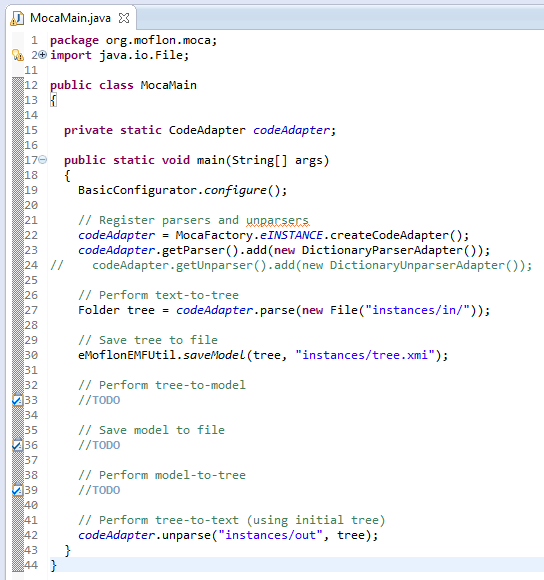
\includegraphics[width=\textwidth]{eclipse_dictionaryMocaMain}
  \caption{Generated main method}
  \label{eclipse:mocaMain} 
\end{center}
\end{figure}

Go ahead and look at what this \texttt{codeAdapter} does. All the code can be adjusted and used, for example, to define which files the parser is
to be used for (per default the adapter registers for \texttt{*.dictionary} files). The main job of the adapter is to hide \texttt{ANTLR} specifics so the
framework remains (parser) technology agnostic. If you decide to use a different parser generator or write the parser by hand you would need to implement a
corresponding adapter from scratch.

On line 27, the input for the framework is set, meaning that all folders in \texttt{./instances/in} are parsed.
In a nutshell, each folder is taken as a root of a tree and the folder and file structure is reflected as a hierarchy of (children) nodes in the tree.
For each file, the framework searches for a registered parser that is responsible for the particular file, passes the content on to the parser and plugs in the
tree from the parser as a single subtree of the corresponding file node in the overall tree.  

\newpage

The final step is now to prepare some input for the framework:
\begin{enumerate}

\item[$\blacktriangleright$] Navigate to ``DictionaryCodeAdapter/instances/in'' and create the directory structure depicted in Fig.~\ref{}. You can create
the \texttt{dictionary} files by right clicking its parent folder, going to ``new/File" and simply appending \texttt{.dictionary} to the end of the name.
Complete each of the four files with the contents from Table~\ref{moca-inputdata}.\footnote{Please do not copy and paste this data as it your .pdf reader may
add some invisible characters to the file that MOSL cannot detect}
 
\begin{figure}[htp]
\begin{center}
  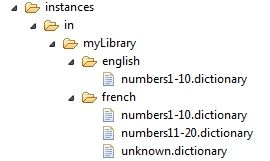
\includegraphics[width=0.5\textwidth]{inputData}
  \caption{Input directory structure.}
  \label{fig:moca-inputdata}
\end{center}
\end{figure}

\end{enumerate}

\begin{table}
\begin{tabular}{p{6cm} p{6cm} }
\footnotesize
\textbf{english/numbers1-10.dictionary:}
\begin{verbatim}
title: "English Numbers 1-10"
email: "contact@langenscheidt.de"	
{
  "null : zero", beginner
  "eins : one", beginner
  "zwei : two", beginner
  "drei : three", beginner
  "vier : four", beginner
  "fuenf : five", beginner
  "sechs : six", beginner
  "sieben : seven", beginner
  "acht : eight", beginner
  "neun : nine", beginner
  "zehn : ten", beginner 
}
\end{verbatim} 

\footnotesize
\textbf{french/numbers11-20.dictionary:}
\begin{verbatim}
title: "French Numbers 11-20"
email: "contact@pons.de"	
{
  "elf : onze", advanced
  "zwoelf : douze", advanced
  "dreizehn : treize", advanced
  "vierzehn : quatorze", advanced
  "fuenfzehn : quinze", advanced
  "sechzehn : seize", master
  "siebzehn : dix-sept", master
  "achtzehn : dix-huit", master
  "neunzehn : dix-neuf", master
  "zwanzig : vingt", master
}
\end{verbatim}
&

\footnotesize
\textbf{french/numbers1-10.dictionary:}
\begin{verbatim}   
title: "French Numbers 1-10"
email: "contact@pons.de"	
{
  "null : zero", beginner
  "eins : un/une", beginner
  "zwei : deux", beginner
  "drei : trois", beginner
  "vier : quatre", beginner
  "fuenf : cinq", beginner
  "sechs : six", beginner
  "sieben : sept", beginner
  "acht : huit", beginner
  "neun : neuf", beginner
  "zehn : dix", beginner 
}
\end{verbatim}

\footnotesize
\textbf{french/unknown.dictionary:}
\begin{verbatim}
title: "unknown"
{
  "unbekannt", beginner
}
\end{verbatim}
  \\
\end{tabular}   
\caption{Input files containing dictionaries.}
\label{moca-inputdata}

\end{table}   

After saving each of the dictionaries, right-click on \texttt{MocaMain.java} and navigate to ``Run As / Java Application.'' If any errors appear in the
``Problems'' tab below the editor, double check that there are no extra spaces in any of the dictionary for lexer files. If everything succeeds, a
\texttt{tree.xmi} file and an \texttt{out} folder (with the same directory structure as \texttt{in}) should be created in the \texttt{instances} directory after
refreshing.

\newpage

Inspect the folder contents and compare them to Fig.~\ref{eclipse_postParse}. The unparsed files are obviously empty as we haven't implemented an
\emph{unparser} yet. Don't be irritated by the fact that an identical \texttt{out/in} pair is created -- this can all be configured in \texttt{MocaMain}. The
default assumes \texttt{in} contains multiple folders (in our case, libraries) and is therefore treated as the root of the tree. One could unparse directly in
\texttt{instances}, but the unparsed \texttt{in} would then have to be renamed in \texttt{MocaMain}.

\vspace{0.5cm}

\begin{figure}[!htbp]
\begin{center}
 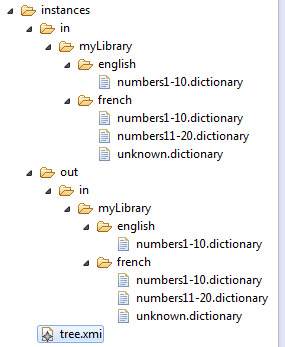
\includegraphics[width=0.4\textwidth]{eclipse_instancesPostParse}
  \caption{Directory \texttt{instances} after parsing}
  \label{eclipse_postParse}
\end{center}
\end{figure} 

\begin{enumerate}

\item[$\blacktriangleright$] Double-click \texttt{tree.xmi} and compare the contents to Fig.~\ref{eclipse:treeResult}. At this point, you can reflect on the
structure of the tree and note the directory structure, file nodes and the subtrees from the parser. This file is important to understand; The directory
structure is transformed to a corresponding hierarchy of \texttt{Folders} and \texttt{Files}. The actual \emph{textual content} of each file is then transformed
to a subtree using a registered, suitable parser. The resulting subtree from the parser is then plugged into the tree by setting its root as the single child
node of a \texttt{File}.

\end{enumerate}

If everything worked out, well done! You now have a nicely structure tree that we'll be able to use with TGGs and transform in a few simple steps into an actual
instance of our \texttt{Dictionary} metamodel.

\newpage

\vspace*{2cm}

\begin{figure}[!htbp]
\begin{center}
 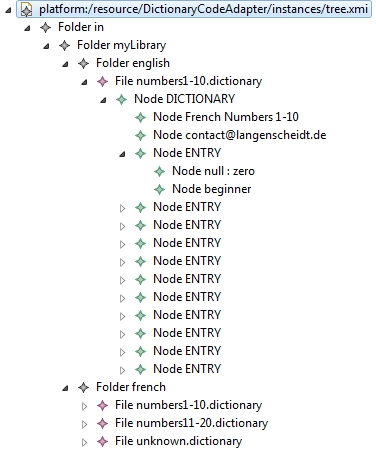
\includegraphics[width=0.55\textwidth]{eclipse_treeParseResult}
  \caption{MocaTree created by the framework using our parser}
  \label{eclipse:treeResult}
\end{center}
\end{figure}

